\documentclass{article}
\usepackage[utf8]{inputenc}
\usepackage{tikz}

\title{TikZ}
\author{Pontus Vikstål}
\date{April 2019}

\begin{document}

%\maketitle

\newcommand\encircle[1]{%
  \tikz[baseline=(X.base)]
    \node (X) [draw, shape=circle, inner sep=0] {\strut #1};}

\section{Introduction}

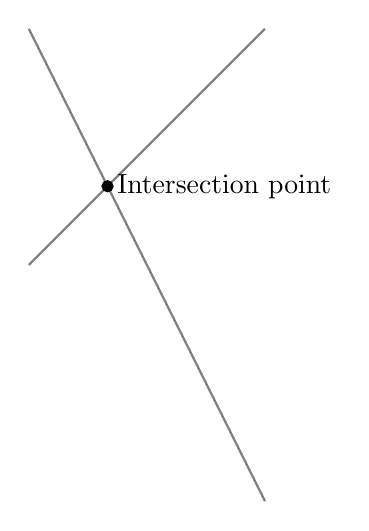
\begin{tikzpicture}
\draw[gray, thick] (-1,2) -- (2,-4);
\draw[gray, thick] (-1,-1) -- (2,2);
\filldraw[black] (0,0) circle (2pt) node[anchor=west] {Intersection point};
\end{tikzpicture}


\begin{tikzpicture}
\draw (-2,0) -- (2,0);
\filldraw [gray] (0,0) circle (2pt);
\draw (-2,-2) .. controls (0,0) .. (2,-2);
\draw (-2,2) .. controls (-1,0) and (1,0) .. (2,2);
\end{tikzpicture}

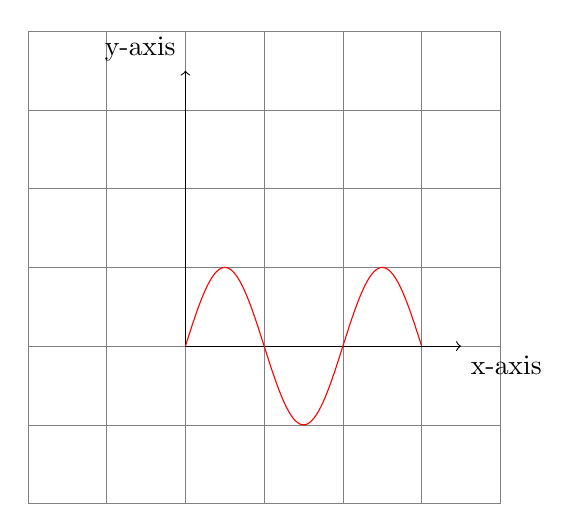
\begin{tikzpicture}
% grid
\draw [help lines] (-2,-2) grid (4,4);
% coordinate system
\draw[->] (0,0) -- (3.5,0) node[anchor=north west] {x-axis};
\draw[->] (0,0) -- (0,3.5) node[anchor=south east] {y-axis};

% draw a sine curve. The trigonometric functions assume that x is in degrees; to express x in radians follow it with the notation "r"
\draw [red, domain=0:3, samples=100] plot (\x, {sin(pi*\x r)});

\end{tikzpicture}

% Bloch sphere
\begin{tikzpicture}[scale=1]

  % Define radius
  \def\r{2}

  % Sphere
  \draw (orig) circle (\r); % circle
  \draw[thick,dashed] (orig) ellipse (\r{} and \r/3); % ellipse

  % Bloch vector
   \draw (0,0) node[circle,fill,inner sep=1] (orig) {} -- (\r/3,\r/2) node[circle,fill,inner sep=0.7,label=above:$|\psi\rangle$] (a) {};
   \draw[dashed] (orig) -- (\r/3,-\r/5) node (phi) {} -- (a);

  % Coordinate system
  \draw[->] (orig) -- ++(-\r/5-.5,-\r/3-.5) node[below] (x1) {$x$};
  \draw[->] (orig) -- ++(\r+.5,0) node[right] (x2) {$y$};
  \draw[->] (orig) -- ++(0,\r+.5) node[above] (x3) {$z$};

  % Angles
  \pic [draw=gray,text=gray,->,"$\phi$"] {angle = x1--orig--phi};
  \pic [draw=gray,text=gray,<-,"$\theta$"] {angle = a--orig--x3};

  % Computational basis states
  \filldraw[fill=white] (0,2) circle (2pt) node[anchor=south west] {$|0\rangle$};
  \filldraw[fill=white] (0,-2) circle (2pt) node[anchor=north west] {$|1\rangle$};

\end{tikzpicture}
\end{document}
